\documentclass{article}
\usepackage{tikz}
\begin{document}

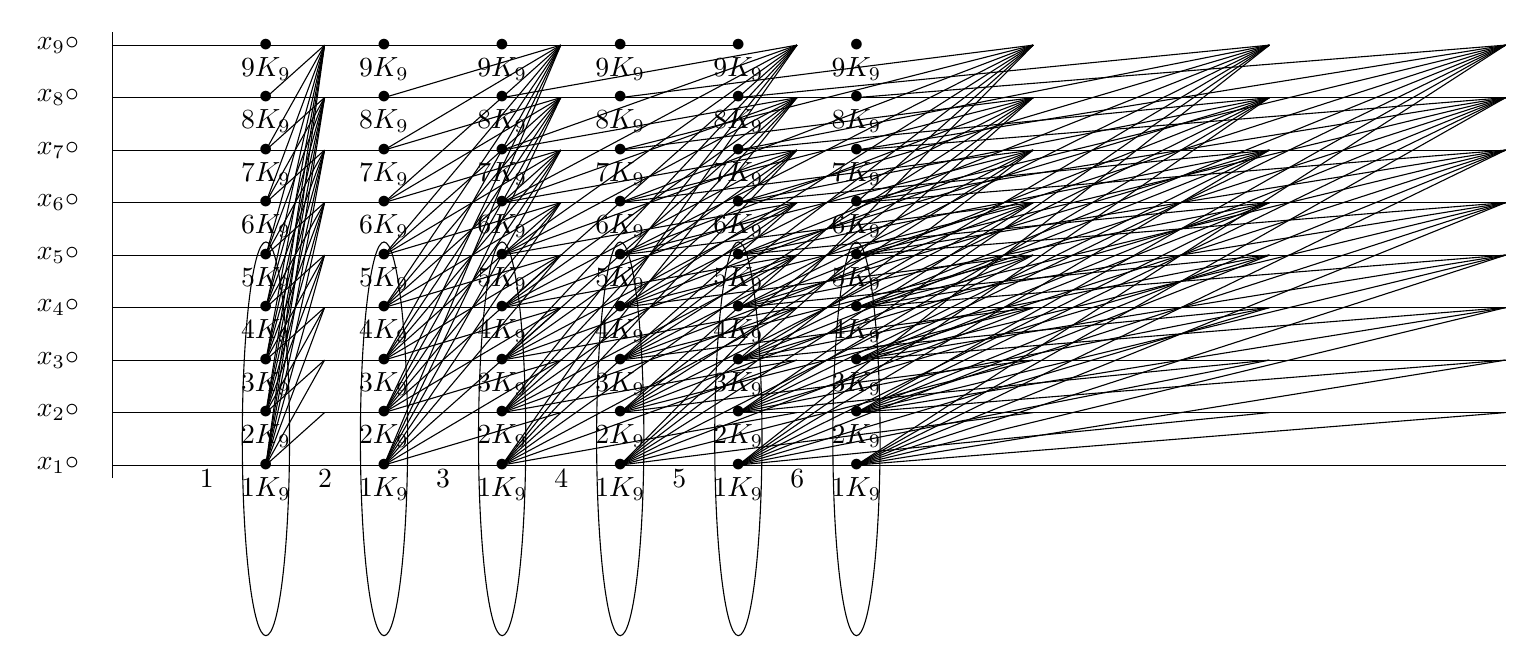
\begin{tikzpicture}
    % Draw the vertex labels for the left-hand side
    \foreach \y/\txt in {
        9/{$x_9$},
        8/{$x_8$},
        7/{$x_7$},
        6/{$x_6$},
        5/{$x_5$},
        4/{$x_4$},
        3/{$x_3$},
        2/{$x_2$},
        1/{$x_1$}}
        \node[anchor=east] at (0, \y/1.5-1) {\txt $\circ$};
    
    % Draw the vertical line on the left
    \draw (0.3, -0.5) -- (0.3, 8.5/1.5-0.5);
    
    % Draw the groups of vertices on the right
    \foreach \x in {1,...,6} {
        \begin{scope}[xshift=\x*1.5cm]
            % Draw the vertical ellipses
            \draw (0.75, 0) ellipse [x radius=0.3, y radius=2.5] ;
            
            % Draw the vertices
            \foreach \y in {1,...,9} {
                \node at (0.75, \y/1.5-1) {$\bullet$};
                \node at (0.75, \y/1.5-1.3) {\y$K_9$}; % Label each group
                \ifnum \y<9
                    \foreach \dy in {\y,...,9} {
                        \draw (0.75, \y/1.5-1) -- (0.15+\x*1.5cm-0.3, \dy/1.5-1);
                    }
                \fi
            }
        \end{scope}
    }
    
    % Label the bottom axis
    \foreach \x/\txt in {1/1, 2/2, 3/3, 4/4, 5/5, 6/6}
        \node at (\x*1.5, -0.5) {\txt};

    % Draw the horizontal lines between left vertices and right vertices
    \foreach \y in {1,...,9} {
        \foreach \x in {1,...,6} {
            \draw (0.3, \y/1.5-1) -- (\x*1.5-0.75, \y/1.5-1);
        }
    }
\end{tikzpicture}

\end{document}